
\documentclass[conference]{IEEEtran}

\usepackage{float} 
\usepackage{url}  
\usepackage{multirow}
\usepackage{caption}
\usepackage{subcaption}
\usepackage{booktabs}
\usepackage{cite}
\pagestyle{plain}
\usepackage{amsmath}
\usepackage{float}
\usepackage{tikz}
\usetikzlibrary{shapes.geometric, arrows, positioning}
\usepackage{placeins}
\usepackage{comment}
\usepackage{tabularx}
\ifCLASSINFOpdf
  \usepackage[pdftex]{graphicx}
\fi

\hyphenation{op-tical net-works semi-conduc-tor}

\begin{document}


\title{tiutlo titlo titlo}

\author{\IEEEauthorblockN{\\ Hugo Veríssimo}
\IEEEauthorblockA{Complements of Machine Learning 24/25\\
University of Aveiro\\
Aveiro, Portugal\\
hugoverissimo@ua.pt}
\and
\IEEEauthorblockN{\\ João Cardoso}
\IEEEauthorblockA{Complements of Machine Learning 24/25\\
University of Aveiro\\
Aveiro, Portugal\\
joaopcardoso@ua.pt}}

\maketitle
\thispagestyle{plain}

\begin{abstract}
abstratotoototot
\end{abstract}

\begin{quote}
\small
\noindent
\textbf{Keywords:} key, word, number, 1
\end{quote}

\IEEEpeerreviewmaketitle


\section{Introduction}

intro

\section{State of The Art}

sota 

\section{Methodology}

\subsection{Dataset \& EDA}

The Financial PhraseBank is a widely used benchmark dataset for financial sentiment analysis. It consists of roughly 4,840 English sentences (mostly news headlines or short statements) about companies, drawn from financial news articles and press releases. Each sentence is labeled with one of three sentiment classes – positive, negative, or neutral – representing the sentence’s sentiment from the perspective of an investor.

+ 50 66 75 percento

ns q concordancia bla bla

https://huggingface.co/datasets/takala/financial\_phrasebank
\cite{dataset, malo2013gooddebtbaddebt}


\subsection{Preprocessing}

split teste e treino

\section{Models}

abcbdhdhhd

\subsection{model 1}

exemplo de imagem

\begin{figure}[H]
    \centering
    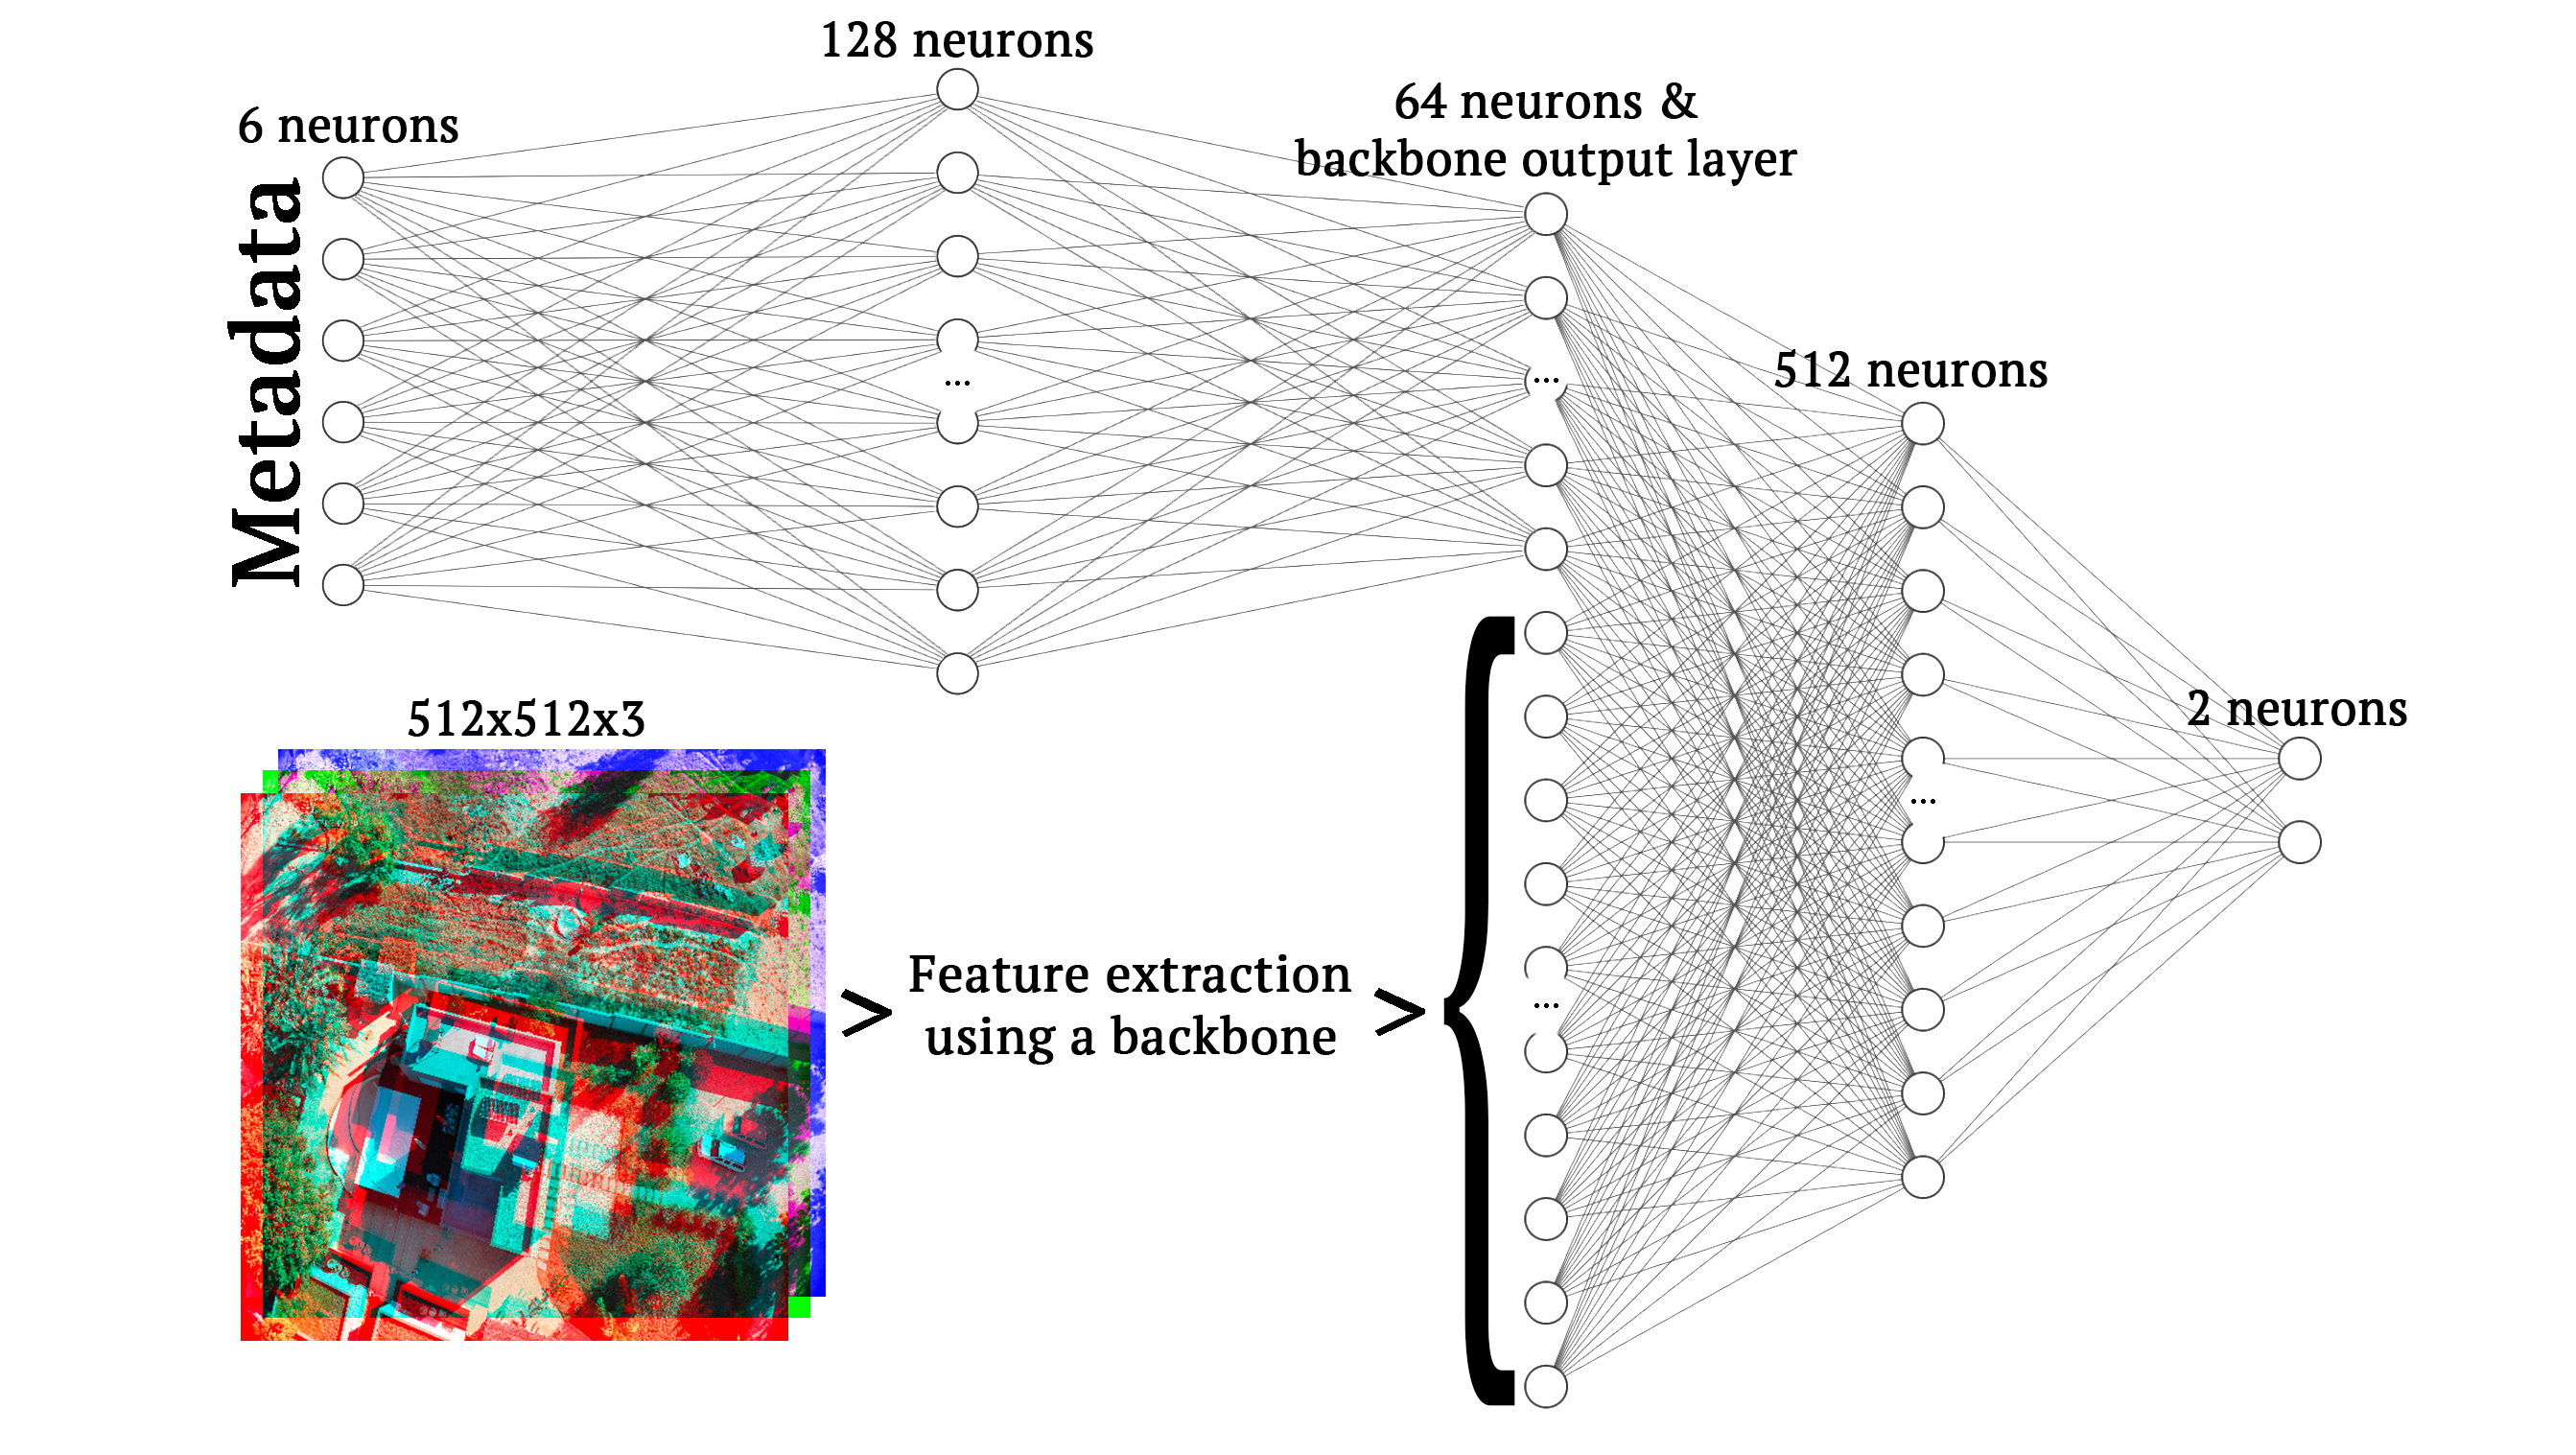
\includegraphics[width=1\linewidth]{assets/nn.png}
    \caption{Architecture of the model shared by user zulo40 in the discussion forums.}
    \label{fig:nn}
\end{figure}

hyp tunning example

\begin{table}[H]
\centering
\caption{Hyperparameter space for the models based of the hybrid model \textit{zulo40}. The bold values correspond to the selected hyperparameters.}
\label{parametroszulp}
\begin{tabular}{ll}
\toprule
\textbf{Hyperparameter} & \textbf{Possible Values} \\
\midrule
Batch size & $\{\mathbf{16}, 32, 64\}$ \\
Optimizer & \textbf{AdamW} \\
Learning rate & $[\mathbf{10^{-5}}, 10^{-3}]$ \\
Weight decay & $[\mathbf{10^{-5}}, 10^{-3}]$ \\
Dropout & $\{0.2, 0.3, \mathbf{0.4}\}$ \\
Scheduler & \textbf{CosineAnnealingWarmRestarts} \\
T\_0 & $\{3, \mathbf{5}, 7, 10\}$ \\
T\_mult & $\{1, \mathbf{2}, 3, 5\}$ \\
Loss & \textbf{HuberLoss} \\
$\delta$ & \textbf{1} \\
\bottomrule
\end{tabular}
\end{table}


\subsection{model 2}

model 2

\subsection{model 3}

model 3

\section{Discussion}

results discuttion

eemplo de comparacao

\begin{table}[H]
\centering
\caption{Error metric (MAE) for the fine-tuned models, along with the best performers in the competition.}
\label{tab:model02_results_transposed}
\begin{tabular}{lr}
\toprule
\textbf{Model} & \textbf{MAE (Test Set)} \\
\midrule
Hybrid & 0.8434 \\
Obj. Det. & 1.2645 \\
Inst. Seg. & 1.3415 \\
Team Lacuna (1st) & 0.3299 \\
K\_Junior (2nd) & 0.5698 \\
\bottomrule
\end{tabular}
\end{table}




\section{Conclusion}

conclisao


\section*{Work Load}

Both authors contributed equally to the project.

\bibliographystyle{IEEEtran}
\bibliography{references}

\end{document}



